\section{任务四}

\subsection{实验目标与攻击思路}

本任务在给定的第3.1.2.4节五轮CipherFour差分密钥恢复攻击程序上进行修改，
保留读取数据、构造明文对、去噪、逆S盒部分解密与候选计数的流程，
使用任务一所选的四轮差分
\[
    \Delta_{\mathrm{in}}=\texttt{0x0001}
    \quad\longrightarrow\quad
    \Delta_{\mathrm{out}}=\texttt{0x0010}
\]
对五轮 CipherFour 进行差分密钥恢复攻击。攻击使用给定的
\texttt{plaintext.txt} 和 \texttt{ciphertext.txt} 中一一对应的明密文，
恢复最后一个轮密钥 $K_5$ 的一个 4 比特半字节。

五轮算法使用六个 16 比特轮密钥 $K_0,\ldots,K_5$。
前四轮包含轮密钥异或、S 盒替换及 P 置换，第五轮不包含 P 置换。
设前四轮的输出为 $U_4$，则最终密文为
\[
    C=S(U_4\oplus K_4)\oplus K_5.
\]
其中，$S$ 表示对四个半字节并行应用 S 盒。

目标四轮输出差分为 \texttt{0x0010}，因此第五轮只有从左到右的
第三个 S 盒活跃，其输入差分为 1。将半字节从左到右编号为
$0,1,2,3$，攻击目标为 $k_{5,2}$，其提取方式为
\[
    k_{5,2}=(K_5\gg4)\mathbin{\&}\texttt{0xF}.
\]

\subsection{明文配对与去噪条件}

首先建立明文到密文的对应表，对每个明文 $x$ 查找
$x'=x\oplus\texttt{0x0001}$，得到对应的密文对 $(C,C')$。
实验采用有序对计数，对完整的 16 比特码本共得到 $2^{16}$ 个有序对。

根据本实验 S 盒的差分分布表，输入差分为 1 时，可能的输出差分为
\[
    \{1,2,5\}.
\]
对于满足四轮输出差分 \texttt{0x0010} 的正确对，第五轮三个非活跃
S 盒的输出差分仍为零，活跃 S 盒的输出差分属于上述集合。
由于第五轮无 P 置换，最终密文差分必须满足
\[
    C\oplus C'\in
    \{\texttt{0x0010},\texttt{0x0020},\texttt{0x0050}\}.
\]
程序据此筛选密文对。等价地，可以先检查
\[
    (C\oplus C')\mathbin{\&}\texttt{0xFF0F}=0,
\]
再检查活跃半字节的差分是否属于 $\{1,2,5\}$。

该条件是正确对必须满足的必要条件，因此正确对都会保留；
部分不满足目标四轮差分的错误对也可能通过筛选，需要在后续密钥评分时处理。

\subsection{六组密钥下的去噪实验}

首先使用题目指定的六个轮密钥
\[
    (\texttt{0123},\texttt{4567},\texttt{89AB},
     \texttt{CDEF},\texttt{FEDC},\texttt{BA98}),
\]
随后使用随机种子 \texttt{20261001} 另外生成五组不同的密钥。
每组密钥均包含六个 16 比特密钥字，具体取值见图~\ref{fig:task4_result}。

对每组密钥，穷举全部 $2^{16}$ 个有序明文对，记录第四轮输出和最终密文。
记去噪后保留的对数为 $M_j$，其中满足第四轮输出差分
\texttt{0x0010} 的正确对数为 $T_j$，则正确对占比为
\[
    \rho_j=\frac{T_j}{M_j}.
\]
这里的 $T_j$ 通过已知密钥的加密仿真及第四轮中间状态获得，
仅用于评估去噪效果；对给定明密文进行密钥攻击时，评分程序不使用这些中间状态。
程序运行结果如图~\ref{fig:task4_result} 所示。

\begin{figure}[H]
    \centering
    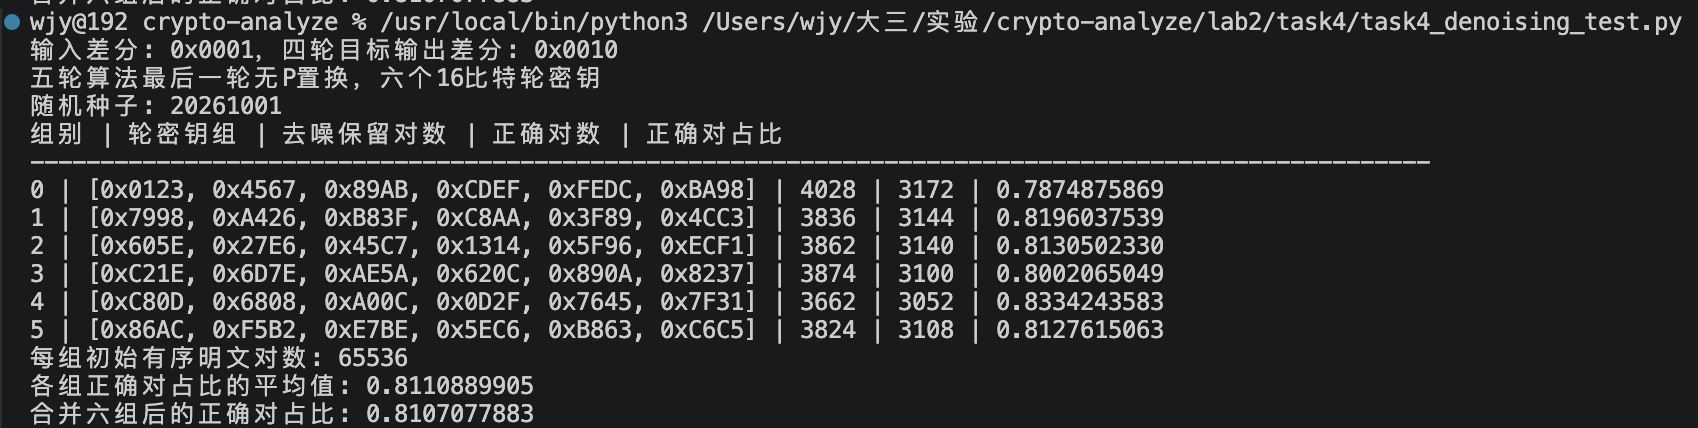
\includegraphics[width=0.95\textwidth]{figures/task4_result.png}
    \caption{六组密钥下的去噪测试结果}
    \label{fig:task4_result}
\end{figure}

六组正确对占比的算术平均为$\textbf{81.1089\%}$，
若合并六组实验的全部保留对，则正确对占比为$\textbf{81.0708\%}$，
两种统计均表明，去噪后保留的明文对中约有 $81\%$ 满足目标四轮差分。

\subsection{最后一轮部分解密与密钥评分}

提取密文的活跃半字节
\[
    c=(C\gg4)\mathbin{\&}\texttt{0xF},
    \qquad c'=(C'\gg4)\mathbin{\&}\texttt{0xF}.
\]
对 $h\in\{0,1,\ldots,15\}$ 逐一猜测 $k_{5,2}$，计算
\[
    v=S^{-1}(c\oplus h),\qquad
    v'=S^{-1}(c'\oplus h).
\]
若 $v\oplus v'=1$，则该猜测得分加一。由于第五轮输入端的
$K_4$ 在差分中抵消，这个判别不需要猜测 $K_4$。

给定文件包含全部 65536 个明文及对应密文。主差分去噪后保留 4028 个
有序对，16 种密钥猜测的得分如表~\ref{tab:task4_scores} 所示。

\begin{table}[H]
    \centering
    \caption{给定明密文的主差分密钥评分}
    \label{tab:task4_scores}
    \renewcommand{\arraystretch}{1.2}
    \begin{tabular}{crcr}
        \toprule
        猜测值 & 得分 & 猜测值 & 得分 \\
        \midrule
        \texttt{0} & 1544 & \texttt{8} & 3172 \\
        \texttt{1} & 1544 & \texttt{9} & 3172 \\
        \texttt{2} & 1268 & \texttt{A} & 1468 \\
        \texttt{3} & 1268 & \texttt{B} & 1468 \\
        \texttt{4} & 1232 & \texttt{C} & 1902 \\
        \texttt{5} & 1232 & \texttt{D} & 1902 \\
        \texttt{6} & 956 & \texttt{E} & 198 \\
        \texttt{7} & 956 & \texttt{F} & 198 \\
        \bottomrule
    \end{tabular}
\end{table}

最高分候选为 $\{\texttt{0x8},\texttt{0x9}\}$，二者得分均为 3172。
本实验 S 盒在输入差分 1 的判别上存在对称性：对于任意 $a,b$，
\[
    S^{-1}(a)\oplus S^{-1}(b)=1
    \quad\Longleftrightarrow\quad
    S^{-1}(a\oplus1)\oplus S^{-1}(b\oplus1)=1.
\]
因此 $h$ 与 $h\oplus1$ 对每一对密文都会给出相同的主差分判别结果。
这种并列无法仅通过增加同类明文对来消除；主差分攻击只能将候选范围
从 16 个缩小为 2 个，不能单独唯一确定全部 4 比特。

\subsection{复杂度分析}

设给定明密文条目数为 $N$，去噪后保留对数为 $M$。
建立明密文对应表、构造输入差分对及去噪扫描需要 $O(N)$ 时间。
枚举 $2^4=16$ 个目标半字节猜测，对每个保留对进行逆S盒部分解密，
评分需要 $O(16M)$ 时间。因此攻击总时间复杂度为
\[
    O(N+16M).
\]
本次 $N=65536$、$M=4028$，共进行
\[
    16\times4028=64448
\]
次候选判别，每次使用两次逆S盒查表，即128896次逆S盒查表。
这些是半字节部分解密操作，不等于完整五轮加密的次数。

本次使用全部 $2^{16}$ 个不同明文的密文，这表示实验实际使用的数据量，
并非攻击所需最少数据量的结论。有序对计数得到 $2^{16}$ 对，
不同无序明文对只有 $2^{15}$ 对。若按无序对去重，所有计数及评分开销
均减半，候选排序不变。程序保存明密文对应表和筛选后的密文对，
空间复杂度为 $O(N)$。

六组密钥的去噪仿真另需进行 $6\times2^{16}$ 次五轮加密。
该部分用于实验评估，应与读取给定明密文后的攻击成本区分。


